%%%%%%%%%%%%%%%%%%%%%%%%%%%%%%%%%%%%%%
%%%%%%%%%%%%%%%%%%%%%%%%%%%%%%%%%%%%%%
% Do not edit the TeX file your work
% will be overwritten.  Edit the RnW
% file instead.
%%%%%%%%%%%%%%%%%%%%%%%%%%%%%%%%%%%%%%
%%%%%%%%%%%%%%%%%%%%%%%%%%%%%%%%%%%%%%



In this section, we apply our methods to Fisher's iris data set, using the
Gaussian mixture model (GMM) model from \exref{iris_bnp_process} and VB
approximation given in \eqref{vb_mf} and \exref{iris_var_distr}.  Here, the data
dimension $d = 4$, we set the truncation parameter $\kmax = 15$.  For our
quantities of interest, we investigate both the estimated number of in-sample
clusters as described in \exref{vb_insample_nclusters_simple} and the
\textit{posterior predictive} number of clusters. Let $\nclusters(\z)$ be the
number of clusters as defined as in \exref{insample_nclusters_simple}.  The
posterior predictive number of clusters, $\expect{\p(\pi \vert
\x)}{\expect{\p(\z \vert \pi)}{\nclusters(\z)}}$, is the posterior expectation
of the number of distinct clusters that we would expect to see in a new dataset
the same size as our original dataset.  Analogously to
\exref{insample_nclusters_simple}, we define a variational approximation to
posterior predictive number of clusters as
%
\begin{align*}
\gclusterspredabbr(\eta) :=
    \expect{\q(\nu\vert\eta)}{\expect{\p(\z\vert\nu)}{\nclusters(\z)}}
  = \sum_{k=1}^\kmax\left(1 -
  \expect{\q(\nu \vert \eta)}{(1 - \pi_\k)^\N} \right).
\end{align*}
%
In the iris example, the predictive quantity can interpreted as the expected
number of species one might see if a fresh sample of iris flowers were
collected.

\subsubsection*{Parametric sensitivity}

We first explore sensitivity of the in-sample and posterior predictive number of
clusters to the concentration parameter, $\alpha$, using the results in
\secref{diffable_concentration}.  To choose a plausible range of $\alpha$,
recall that, under the GEM$(\alpha)$ prior, the {\em a priori} expected
number of distinct clusters in a dataset of size $N$ is given
\citep{jordan:2015:gentleintrodp} by
%
\begin{align}\eqlabel{prior_num_clusters}
\expect{\p(\z \vert \pi)\p(\pi \vert \alpha)}{\nclusters(\z)} =
\sum_{\n = 1}^\N \frac{\alpha}{\alpha + \n - 1}.
\end{align}
%
Using this formula, we take $\alpha\in[0.1, 4.0]$, corresponding to an an {\em a
priori} range of approximately $1.5$ to $15$ clusters.  Over this range, the
shape of the stick-breaking density varies considerably, as shown in
\figref{beta_priors}.  We take $\alpha_0 = 2$, near the middle of the range, and
use the prior $\p(\nuk \vert \alpha_0)$ as the base prior at which we compute
the derivatives for all the results below.  \Figref{iris_fit} shows the
posterior clustering for $\alpha_0$.  For our base prior, the posterior thus
recovers the known ground truth that there are in truth three distinct species.

\todo{Bryan: these should all have the same y-axis scale}

\begin{knitrout}
\definecolor{shadecolor}{rgb}{0.969, 0.969, 0.969}\color{fgcolor}\begin{figure}[!h]

{\centering 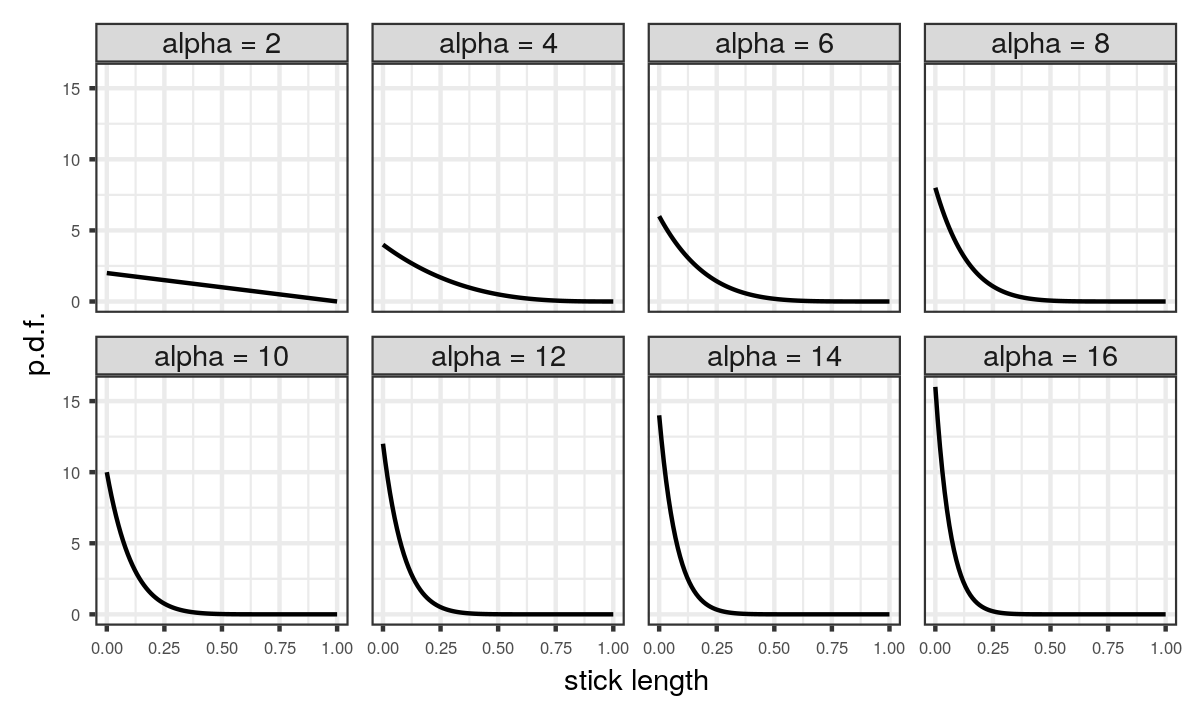
\includegraphics[width=0.980\linewidth,height=0.392\linewidth]{figure/beta_priors-1} 

}

\caption[Probability density functions of $\text{Beta}(1, \alpha)$ distributions, under various $\alpha$ considered for the iris data set]{Probability density functions of $\text{Beta}(1, \alpha)$ distributions, under various $\alpha$ considered for the iris data set.}\label{fig:beta_priors}
\end{figure}


\end{knitrout}


\todo{Bryan: the caption says $\alpha=6$, but the text says $\alpha=2$.}

\begin{knitrout}
\definecolor{shadecolor}{rgb}{0.969, 0.969, 0.969}\color{fgcolor}\begin{figure}[!h]

{\centering 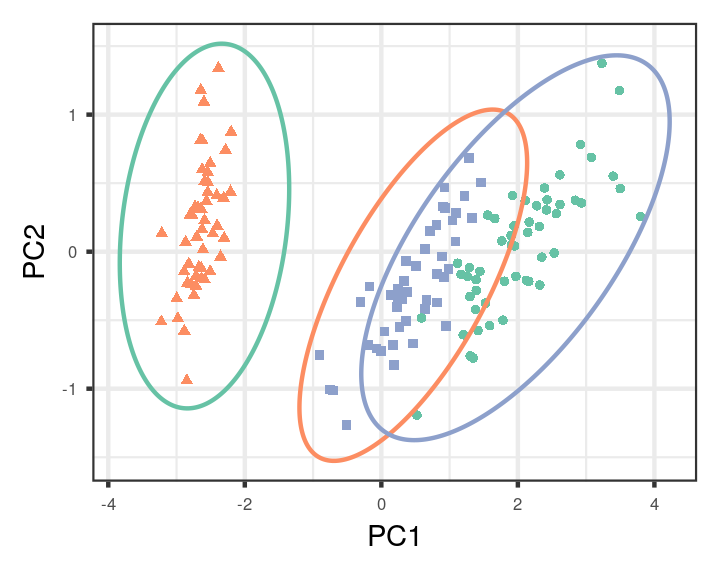
\includegraphics[width=0.588\linewidth,height=0.470\linewidth]{figure/iris_fit-1} 

}

\caption[The iris data in principal component space and
                      GMM fit at $\alpha = 6$.
                      Colors denote inferred memberships and
                      ellipses represent estimated covariances]{The iris data in principal component space and
                      GMM fit at $\alpha = 6$.
                      Colors denote inferred memberships and
                      ellipses represent estimated covariances. }\label{fig:iris_fit}
\end{figure}


\end{knitrout}


\todo{Bryan: Maybe don't hard-code 2 in the caption?}

\begin{knitrout}
\definecolor{shadecolor}{rgb}{0.969, 0.969, 0.969}\color{fgcolor}\begin{figure}[!h]

{\centering 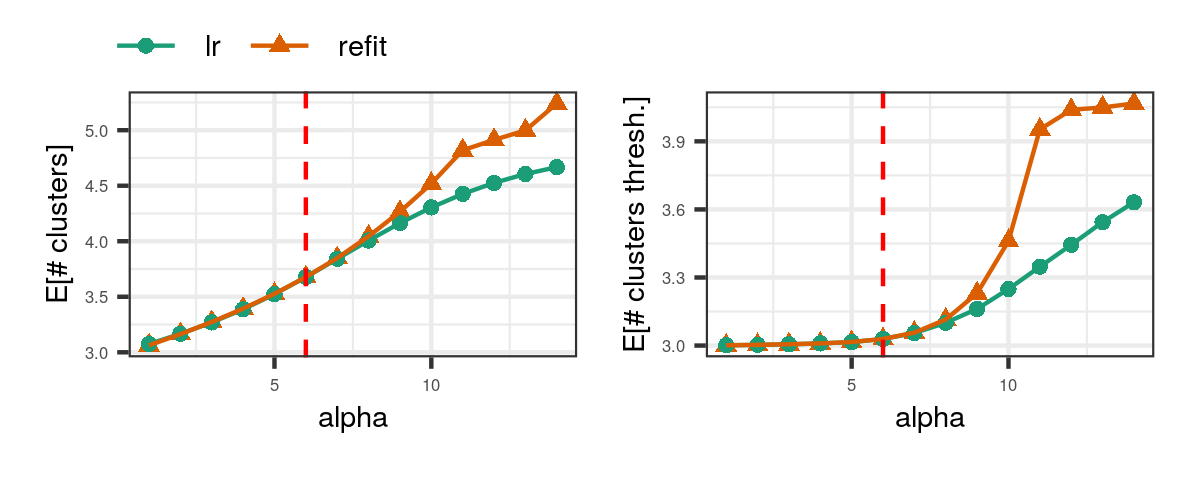
\includegraphics[width=0.784\linewidth,height=0.439\linewidth]{figure/iris_alpha_sens-1} 

}

\caption[The expected number of clusters as $\alpha$ varies in the
the GMM fit of the iris data.
On the left is in-sample quantity $\gclustersabbr$.
On the right is the the predictive quantity $\gclusterspredabbr$.
We formed the linear approximation at $\alpha=2$.
In red, the expected number of clusters computed under the
linearly approximated variational parameters.
In blue, the expected number of clusters obtained by refitting the model at each $\alpha$]{The expected number of clusters as $\alpha$ varies in the
the GMM fit of the iris data.
On the left is in-sample quantity $\gclustersabbr$.
On the right is the the predictive quantity $\gclusterspredabbr$.
We formed the linear approximation at $\alpha=2$.
In red, the expected number of clusters computed under the
linearly approximated variational parameters.
In blue, the expected number of clusters obtained by refitting the model at each $\alpha$. }\label{fig:iris_alpha_sens}
\end{figure}


\end{knitrout}

\Figref{iris_alpha_sens} shows both the posterior in-sample and predictive
number of distinct clusters as $\alpha$ varies.  Over this range of $\alpha$,
the in-sample number of clusters is quite robust, but the posterior predictive
number of clusters is non-robust, ranging roughly from 3.0 to 5.6 expected
species.  Our approximation captures this qualititative behavior. As expected,
the approximation is least accurate furthest from the $\alpha_0$ at which it is
evalutated.

For this dataset, the linear approximation is an order of magnitude faster than
refitting. Forming the linear approximation at $\alpha_0$ required
0.02 seconds. After forming the linear
approximation, computing $\etalinglobal(\alpha)$ for the sequence of $\alpha$'s
considered in \figref{iris_alpha_sens} took another 0.01 seconds. On the other hand, to refit $\etaopt(\alpha)$ for
the set of $\alpha$s took a total of  9 seconds, with a median refit time of
0.5 seconds.

\subsubsection*{Functional perturbations and the influence function}

\todo{Use the notation $\pbase(\nuk) = \betadist(\nuk \vert \alpha=2)$}
We again start with the variational approximation fit with GEM parameter
$\alpha_0 = 2$, but now we consider functional perturbations to
the stick-breaking $\betadist{1, \alpha_0}$ density.
We demonstrate the ability of the influence function to
provide guidance on the anticipated effect of potential perturbations
on the expected number of in-sample clusters.

\todo{This is redundant.  However, you may want to say something
about using a different base measure than our theory examples.}
Recall from \eqref{vb_eta_infl_sens} that the local sensitivity can
be represented as an inner product between the influence function $\infl$
and a multiplicative perturbation $\phi$;
the inner product takes the form,
\begin{align}\eqlabel{recall_infl_innerprod}
\fracat{d g(\etaopt(\t \phi))}{d \t}{0} ={}&
    \int \infl(\lnuk) \phi(\lnuk) \mu(d\lnuk),
\end{align}
where we expressed both the influence function and the perturbation in
unconstrained space, $\lnuk := \log(\nuk) - \log(1 - \nuk)$.
The left column of \figref{iris_fsens} shows the influence function
for the number of in-sample clusters $\gclustersabbr$ in purple.

\todo{A note for everywhere: it's not an inner product.  My bad for calling
it that at some point, but we need to get away from that.  It's just an
integral.  The reason is that the influence function may not be a
member of $L_\infty$; technically, it's a member of the dual space
($L_1$).}
\todo{A lot can be cut by not re-stating things that are already said
in the theory section, and this is another example}
In order to illustrate this inner product,
we consider perturbations $\phi_\mu$
which are Gaussian bumps, with each perturbation centered at a
different $\mu$ on the real line (\figref{iris_fsens} left column).
The perturbed densities are
$p(\lnu_k|\t\phi_\mu) = p_0(\lnu_k)\exp(\t\phi_\mu(\lnu_k))$.
The middle column of \figref{iris_fsens} displays the initial density
$p_0(\nu_k) = \betadist{\nu_k\vert 1, \alpha_0}$
along with the perturbed densities at $\t = 1$
for different choices of $\mu$,
in the original $(0, 1)$ constrained space.

\todo{Left off here...}

% The perturbations of the form
% $\phi_\mu(x) = e^{2(x - \mu)^2}$, with each perturbation having a
% different mode $\mu$ (\figref{iris_fsens} left column).
% The perturbations are multiplicative with perturbed prior
% $p(\nu_k|\t) = p_0(\nu_k)\exp(\t\phi_\mu(\nu_k))$.
% The middle column of \figref{iris_fsens} displays the initial density,
% $p_0(\nu_k) = \betadist{\nu_k\vert 1, \alpha_0}$,
% along with the perturbed densities
% $p(\nu_k|\t = 1)$ for different choices of $\mu$.

Each perturbation $\phi_\mu$ with a different choice of $\mu$
produces distinct changes in the expected number
of in-sample clusters $\gclustersabbr$.
The right column of \figref{iris_fsens} plots the differences
$\Delta\gclustersabbr(\eta(\t)) :=
\gclustersabbr(\eta(\t)) - \gclustersabbr(\etaopt(0))$
for $\t\in[0,1]$.
Depending on the perturbation,
$\Delta\gclustersabbr$ can be positive, negative, or nearly zero.
In each case, the approximation
$\Delta\gclustersabbr(\etalinglobal(\t))$
is able to mirror the qualitative behavior of
$\Delta\gclustersabbr(\etaopt(\t))$
observed by refitting.

While each perturbation produces distinct changes in $\gclustersabbr$,
it is unclear how to anticipate the effect of a perturbation
by comparing the original and perturbed densities alone.
On the other hand, the sign and magnitude of the change in $\gclustersabbr$ after
prior perturbation are well-explained by its influence function
and the representation of local sensitivity as an inner product
(\eqref{recall_infl_innerprod}).
When $\phi_\mu$ is centered at a location where the influence function is negative, the effect of the perturbation on $\gclustersabbr$
is negative (\figref{iris_fsens} top row);
conversely, when $\phi_\mu$ is centered at a location where the influence function is positive, its effect on $\gclustersabbr$ is positive (bottom row);
finally, when $\phi_\mu$ is centered at a location where the influence transitions from negative to positive, its effect on
$\gclustersabbr$ is roughly zero (middle row).
In the last case, $\phi_\mu$ placed approximately equal weight on the negative and positive portions of the prior-weighted influence function, resulting in an approximately zero inner-product.


Finally, we consider the
worst-case multiplicative perturbation with unit $L_\infty$ norm.
Recall that the worst-case perturbation with unit $L_\infty$ norm is a
step-function taking on values $\pm1$ corresponding
to the sign of the influence function (\figref{iris_worstcase} left).
The middle column of \figref{iris_worstcase} shows the prior density perturbed by the worst-case perturbation;
the right column shows the effect on $\gclustersabbr$.
This worst-case perturbation has a much larger effect on
$\gclustersabbr$ compared to the other unit $L_\infty$ norm perturbations in
\figref{iris_fsens}.
However, even with the worst-case perturbation,
the change in $\gclustersabbr$ is still small.
We conclude that on the iris data set, $\gclustersabbr$ appears to be a quantity insensitive to the prior under a Gaussian mixture model.



\begin{knitrout}
\definecolor{shadecolor}{rgb}{0.969, 0.969, 0.969}\color{fgcolor}\begin{figure}[!h]

{\centering 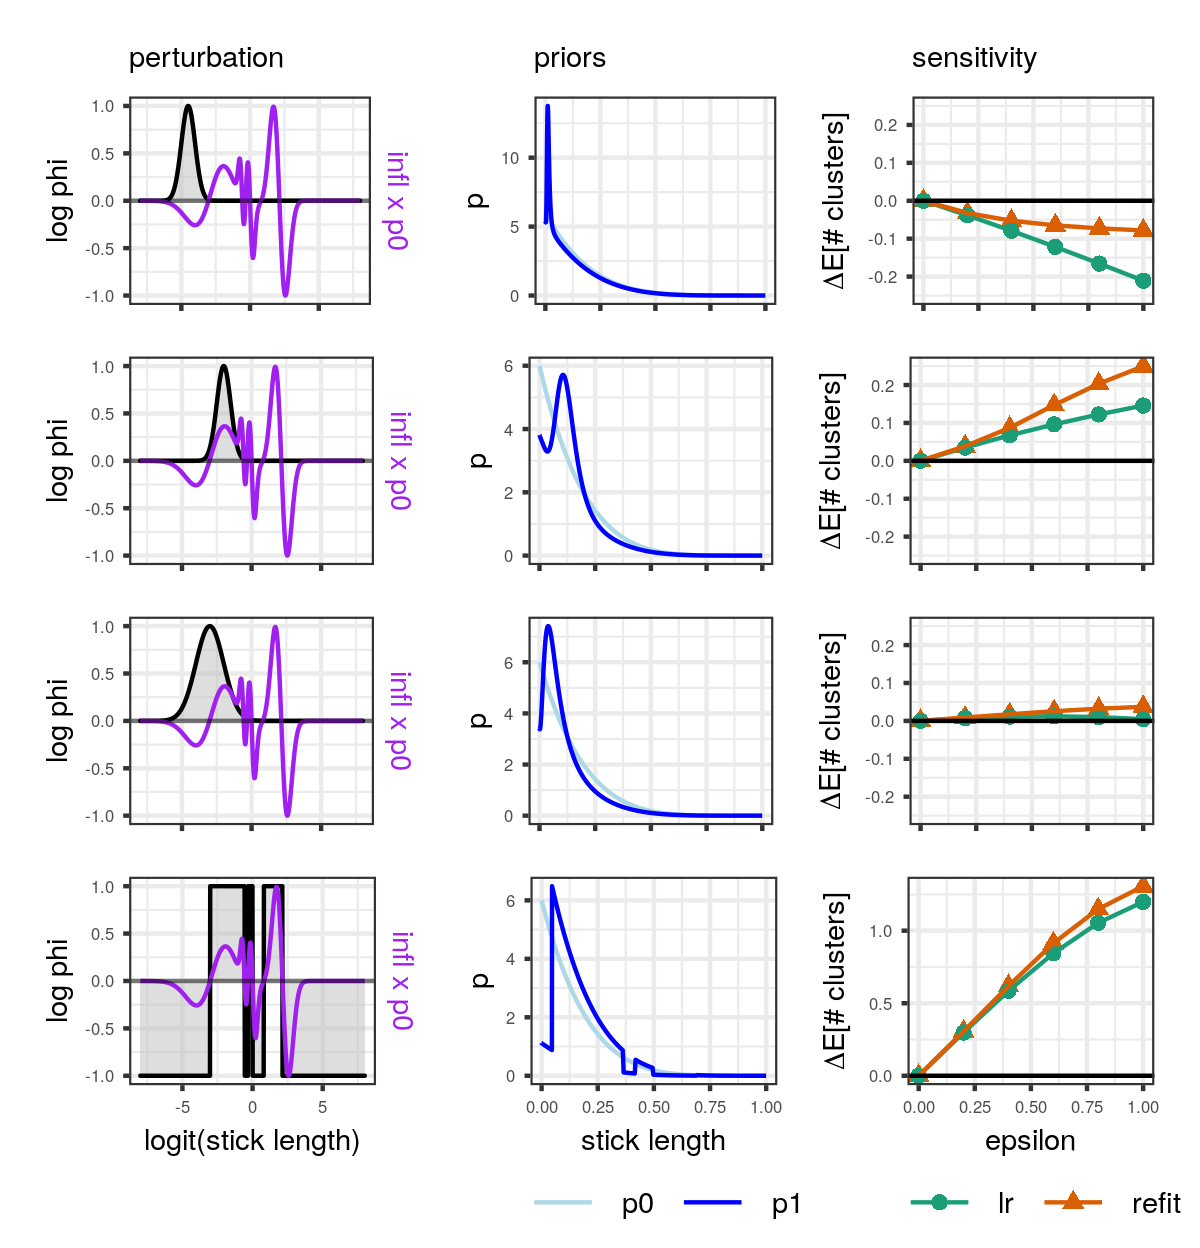
\includegraphics[width=0.980\linewidth,height=0.862\linewidth]{figure/iris_fsens-1} 

}

\caption{Sensitivity of
        the expected number of in-sample clusters
        in the iris data set
        to three multiplicative perturbations with
        unit $L_{\infty}$-norm.
        (Left) the multiplicative perturbation $\phi$ in grey.
        The influence function $\Psi$ in purple,
        scaled to also have unit $L_{\infty}$-norm.
        (Middle) the original prior density $\p_0$ and
        the perturbed prior density $\p_t = \p_0\times \exp(t \phi)$
        at $t = 1$.
        (Right) the effect of the perturbation
        on the change in expected number of in-sample clusters
        as $t\rightarrow1$.}\label{fig:iris_fsens}
\end{figure}


\end{knitrout}


\begin{knitrout}
\definecolor{shadecolor}{rgb}{0.969, 0.969, 0.969}\color{fgcolor}\begin{figure}[!h]

{\centering 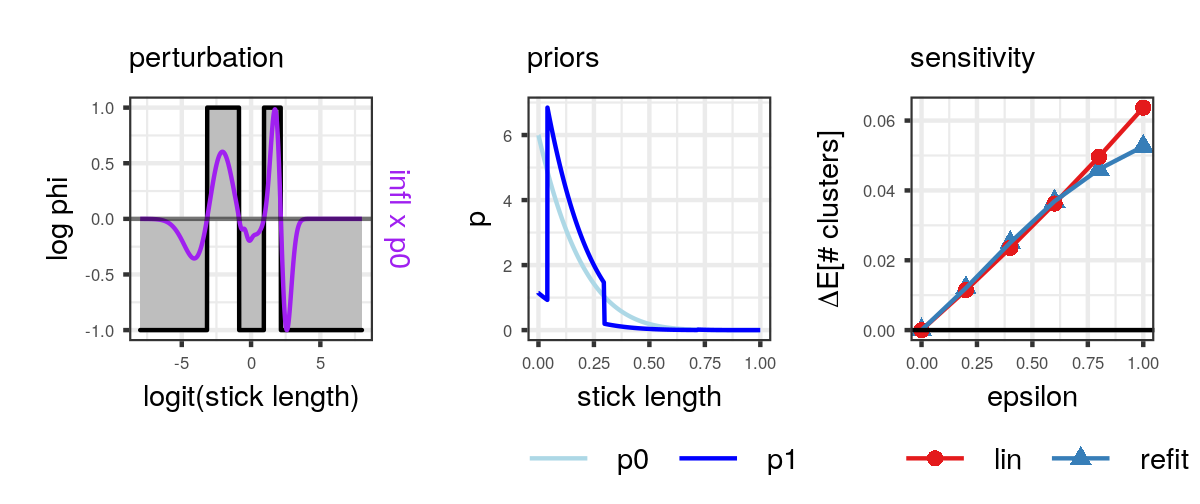
\includegraphics[width=0.980\linewidth,height=0.412\linewidth]{figure/iris_worstcase-1} 

}

\caption[Sensitivity of
        the expected number of in-sample clusters in the iris data set
        to the worst-case multiplicative perturbation with
        unit $L_{\infty}$-norm]{Sensitivity of
        the expected number of in-sample clusters in the iris data set
        to the worst-case multiplicative perturbation with
        unit $L_{\infty}$-norm.}\label{fig:iris_worstcase}
\end{figure}


\end{knitrout}

Computing the linearized variational parameters $\etalinglobal(\t)$ at $\t = 1$
(including the necessary Hessian solve)
for a given functional perturbation
required 0.03 seconds.
A refit at $\t = 1$ requires about one second.
While a second for a refit is not exceedingly large, the
order-of-magnitude difference in timing between the linear approximation and refit
will continue to hold for larger data analysis problems below.
In general, the speed of the linear approximation allows us to quickly
explore many different potential functional perturbations when
refitting for each perturbation becomes prohibitive.
In the data applications below,
the influence function will guide our choice of functional perturbation and
uncover potentially influential perturbations.

% \begin{table}[tb]
% \centering
% \caption{Compute time of results on the iris data set. }
% \begin{tabular}{|r|r|}
%     \hline
%     & time (seconds) \\
%     \hline
%     Initial fit & sprintf('%1.2g', init_fit_time) \\
%     \hline
%     Hessian solve for $\alpha$ sensitivity &
%         sprintf('%1.2g', alpha_hess_time)\\
%     Linear approx. $\eta^{lin}(\alpha)$ for $\alpha = 1, \ldots , 16$ &
%         sprintf('%1.2g', total_alpha_lr_time)\\
%     Refits $\eta(\alpha)$ for $\alpha = 1, \ldots , 16$ &
%         sprintf('%1.2g', total_alpha_refit_time)\\
%     \hline
%     The influence function & sprintf('%1.2g', infl_time)\\
%     Hessian solve for worst-case $\phi$ &
%         sprintf('%1.2g', wc_hessian_time)\\
%     Linear approx. $\eta^{lin}(\t)|_{\t = 1}$
%     for worst-case $\phi$ &
%         sprintf('%1.2g', wc_lr_time)\\
%     Refit $\eta(\t)|_{\t = 1}$ for worst-case $\phi$ &
%         sprintf('%1.2g', wc_refit_time)\\
%     \hline
% \end{tabular}
% \end{table}
